\documentclass{beamer}
\usetheme{Copenhagen}

% Basic packages
\usepackage{subfiles}
\usepackage[quiet]{fontspec}
\usepackage{geometry}
\usepackage{hyperref}
\usepackage{fancyhdr, lastpage}
\usepackage{multirow, multicol}
\usepackage{longtable}
\usepackage{siunitx}
\usepackage{float}
\usepackage{graphicx}
\usepackage{subcaption}

% Hyperref config
\hypersetup{colorlinks=true, urlcolor=blue, linkcolor=white}
\urlstyle{same}

\title{DietDupe}
\subtitle{Explorative data analysis}
\author{Piotr Kaszubski \and Antoni Solarski \and Nina Żukowska}
\institute{Poznań University of Technology}
\date{Monday, November 13, 2023}

\begin{document}
\maketitle
\begin{frame}
	\frametitle{Choosing the dataset}
	\begin{enumerate}
		\item FlavorGraph \href{https://github.com/lamypark/FlavorGraph}{[github]}
			\begin{itemize}
				\item \texttt{FlavorGraph\_node\_embedding.pickle}
				\item \texttt{nodes\_191120.csv}
			\end{itemize}
		\item The Nutritional Content of Food \href{https://www.kaggle.com/datasets/thedevastator/the-nutritional-content-of-food-a-comprehensive}{[kaggle]}
			\begin{itemize}
				\item \texttt{ABBREV.csv}
			\end{itemize}
		\item (future work?) Vegan/non-vegan dataset
	\end{enumerate}
\end{frame}

\begin{frame}
	\frametitle{Dataset -- FlavorGraph}
	\begin{figure}[H]
		\centering
		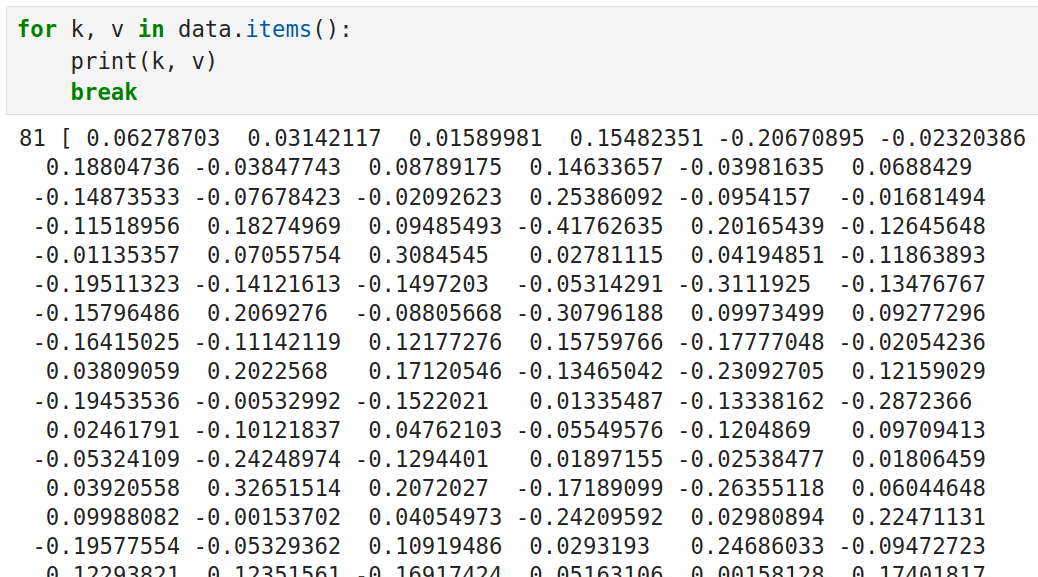
\includegraphics[width=\linewidth]{img/embeddings_head.png}
		\caption{\texttt{FlavorGraph\_node\_embedding.pickle}}
	\end{figure}
\end{frame}

\begin{frame}
	\frametitle{Dataset -- FlavorGraph}
	\begin{figure}[H]
		\centering
		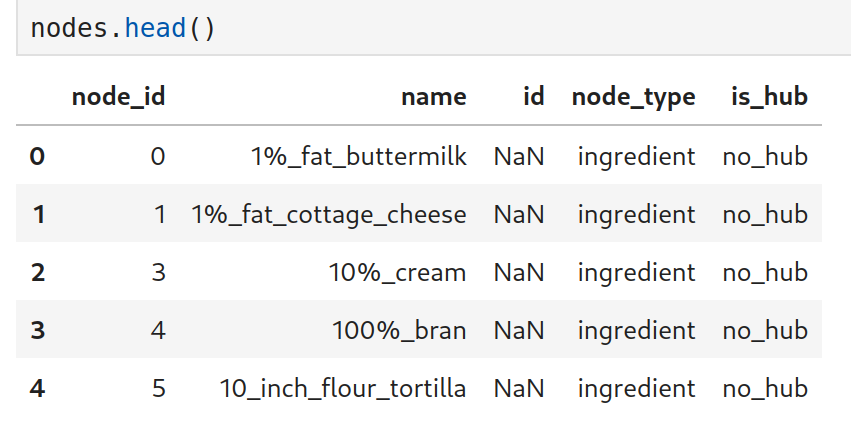
\includegraphics[width=\linewidth]{img/nodes_head.png}
		\caption{\texttt{nodes\_191120.csv}}
	\end{figure}
\end{frame}

\begin{frame}
	\frametitle{Dataset -- The Nutritional Content of Food}
	\begin{figure}[H]
		\centering
		\begin{subfigure}[b]{0.48\linewidth}
			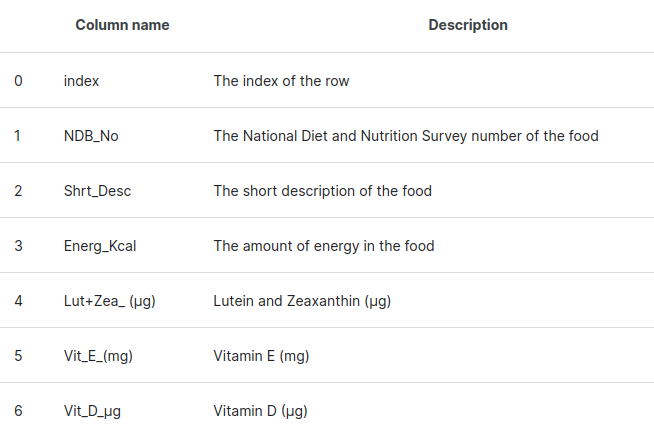
\includegraphics[width=\linewidth]{img/nutri_columns1.png}
		\end{subfigure}
		\begin{subfigure}[b]{0.48\linewidth}
			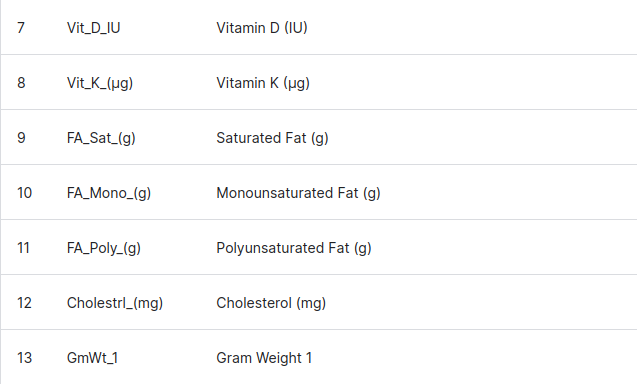
\includegraphics[width=\linewidth]{img/nutri_columns2.png}
		\end{subfigure}
		\caption{\texttt{ABBREV.csv} columns (brief)}
	\end{figure}
\end{frame}

\begin{frame}
	\frametitle{Dataset -- The Nutritional Content of Food}
	\begin{figure}[H]
		\centering
		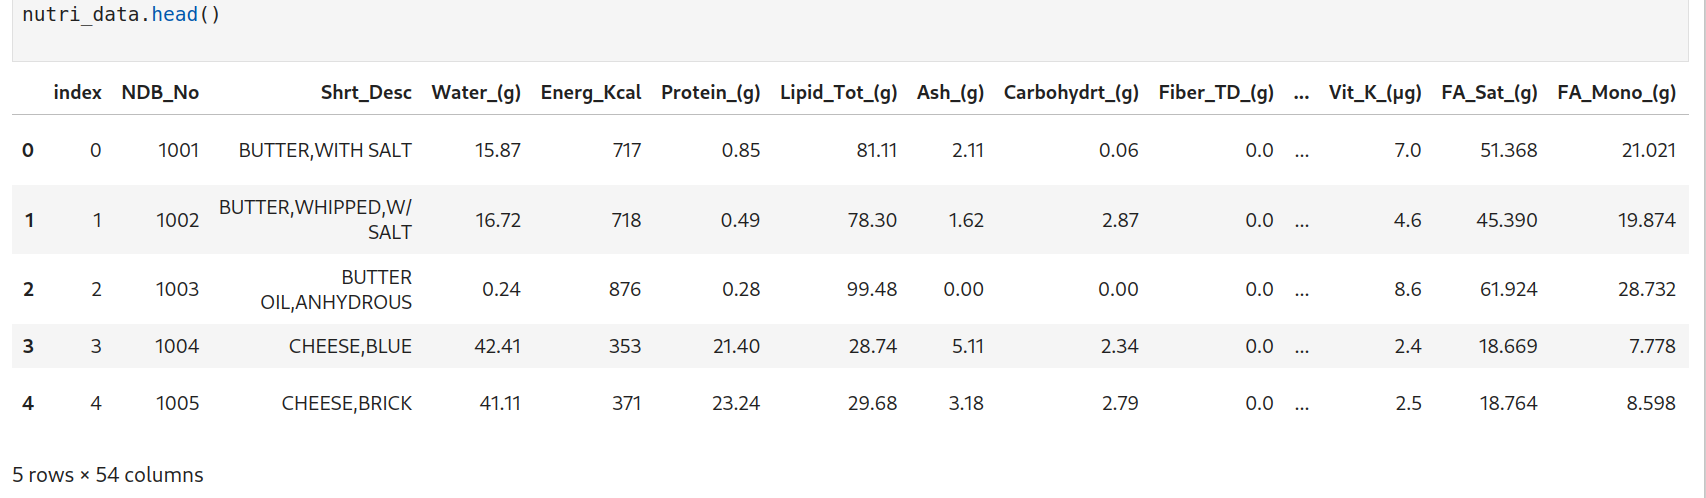
\includegraphics[width=\linewidth]{img/nutri_head.png}
		\caption{\texttt{ABBREV.csv}}
	\end{figure}
\end{frame}

\begin{frame}
	\frametitle{Matching the two datasets}
	\framesubtitle{Method 1: \texttt{BERT}}
	\begin{enumerate}
		\item Use \texttt{BertTokenizer} to transform both datasets into
			same-space embeddings.
		\item Match terms based on cosine similarity.
	\end{enumerate}
	\begin{figure}[H]
		\centering
		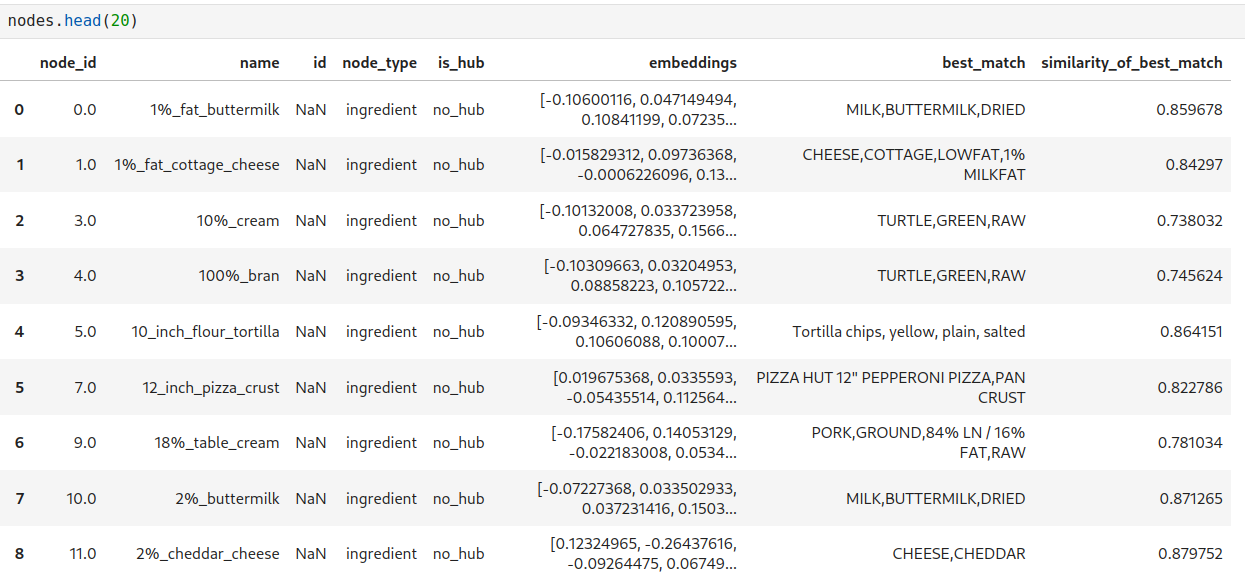
\includegraphics[width=\linewidth]{img/match_bert_head.png}
	\end{figure}
\end{frame}

\begin{frame}
	\frametitle{Matching the two datasets}
	\framesubtitle{Method 2: \texttt{food2vec}}
	\begin{enumerate}
		\item Use \texttt{food2vec.semantic\_nutrition.Estimator} to transform
			both datasets into same-space embeddings.
		\item Match terms based on cosine similarity.
	\end{enumerate}
	\begin{figure}[H]
		\centering
		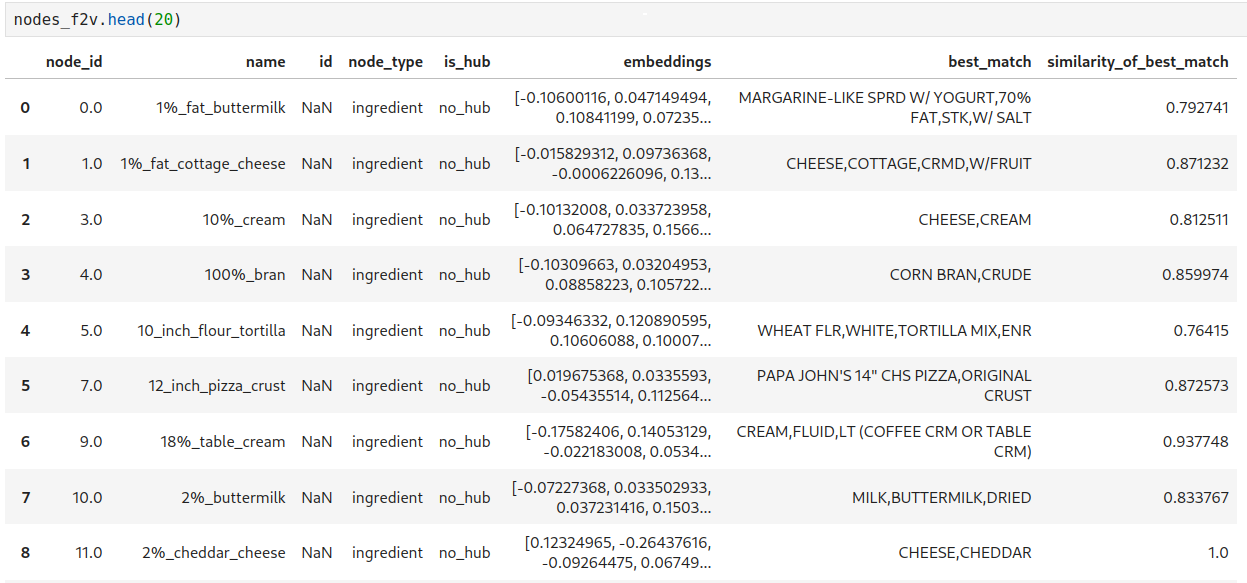
\includegraphics[width=\linewidth]{img/match_f2v_head.png}
	\end{figure}
\end{frame}

\begin{frame}
	\frametitle{Matching the two datasets}
	\framesubtitle{Combining both methods}
	\begin{enumerate}
		\item Fill nodes from \texttt{food2vec} with nodes from \texttt{BERT}.
	\end{enumerate}
	\begin{figure}[H]
		\centering
		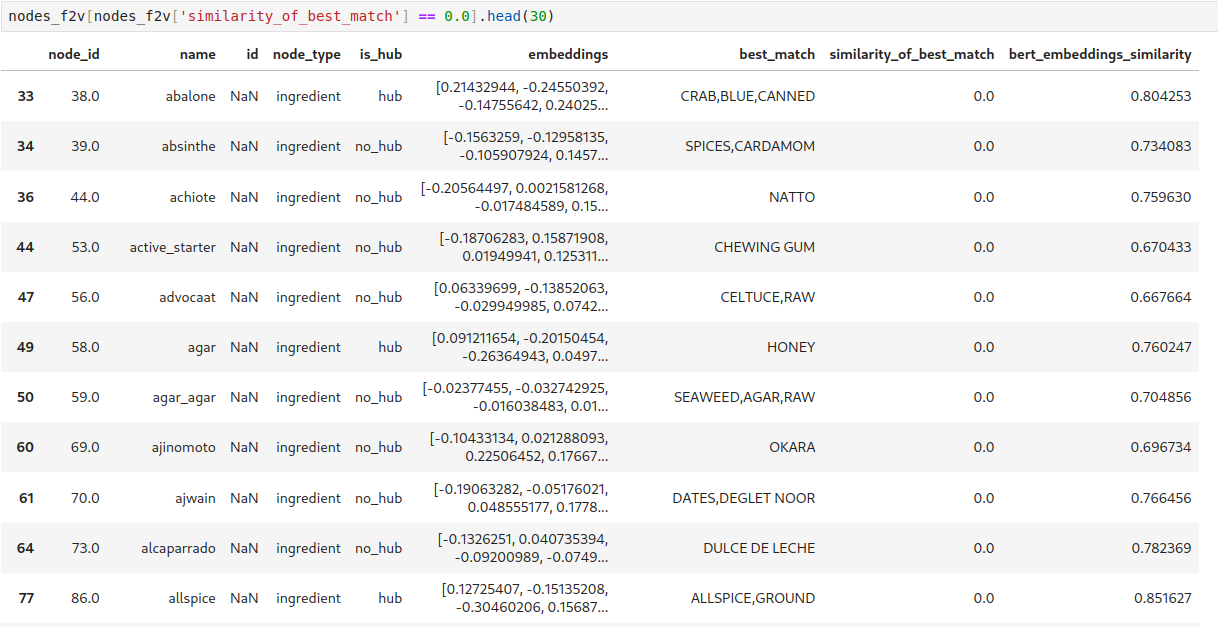
\includegraphics[width=\linewidth]{img/match_combo.png}
	\end{figure}
\end{frame}

\begin{frame}
	\frametitle{Data exploration}
	\begin{figure}[H]
		\centering
		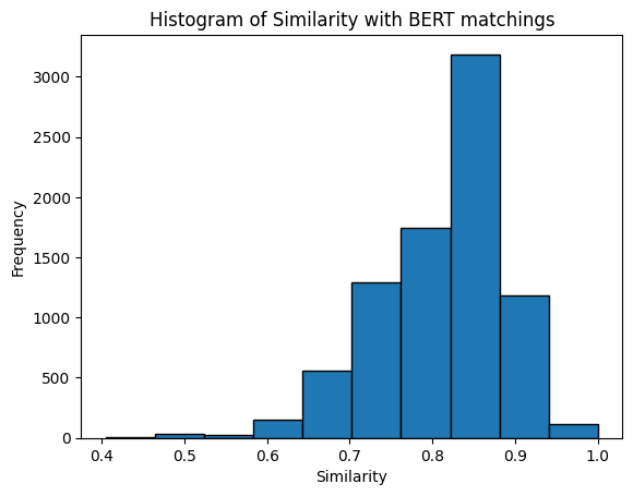
\includegraphics[width=0.9\linewidth]{img/plot_sim_bert.png}
	\end{figure}
\end{frame}

\begin{frame}
	\frametitle{Data exploration}
	\begin{figure}[H]
		\centering
		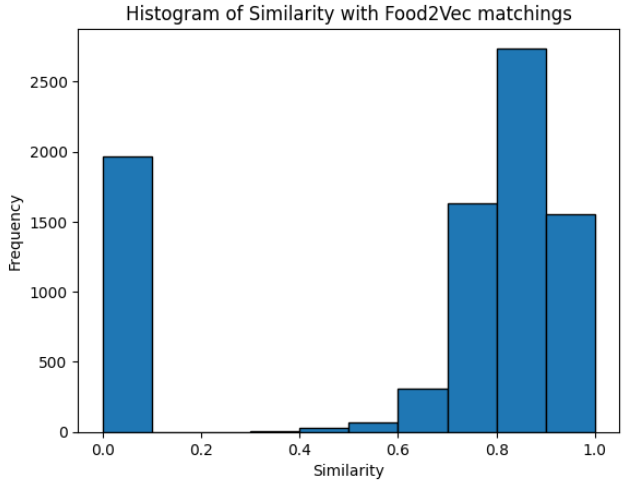
\includegraphics[width=0.9\linewidth]{img/plot_sim_f2v.png}
	\end{figure}
\end{frame}

\begin{frame}
	\frametitle{Data exploration}
	\begin{figure}[H]
		\centering
		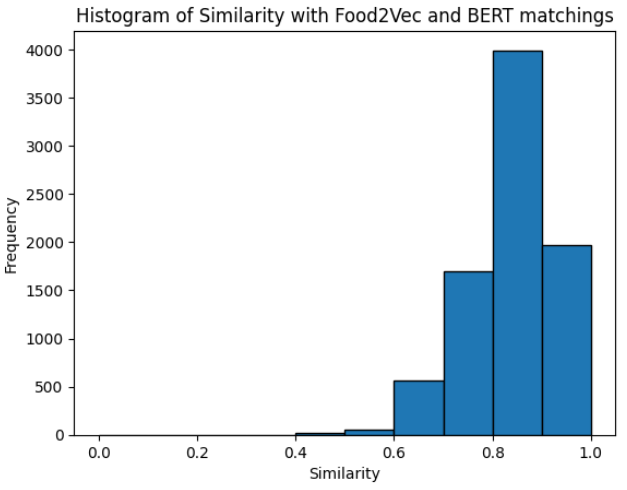
\includegraphics[width=0.9\linewidth]{img/plot_sim_f2v_bert.png}
	\end{figure}
\end{frame}

\begin{frame}
	\frametitle{Data exploration}
	\begin{figure}[H]
		\centering
		\begin{subfigure}[b]{0.45\linewidth}
			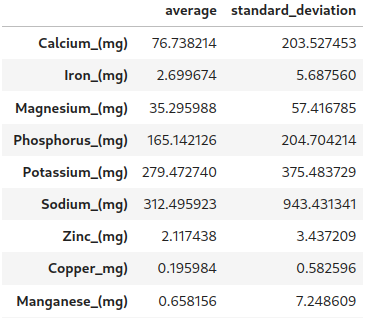
\includegraphics[width=\linewidth]{img/eda_std1.png}
		\end{subfigure}
		\begin{subfigure}[b]{0.45\linewidth}
			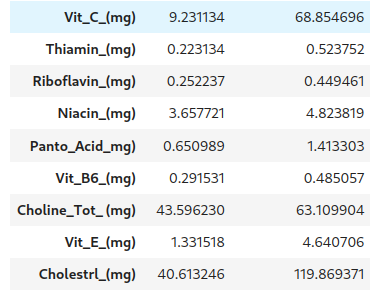
\includegraphics[width=\linewidth]{img/eda_std2.png}
		\end{subfigure}
		\caption{Summary of micronutrient columns}
	\end{figure}
\end{frame}

\end{document}

